\documentclass{article}
\usepackage[utf8]{inputenc}
\usepackage[dutch]{babel}
\setlength
{\parindent}
{0pt}
\setlength
{\parskip}
{1.5ex plus 0.5ex minus 0.2ex}


\title{Gegevensstructuren en Algoritmen: Practicum 1}
\author{Mathias Van Herreweghe }
\date{21 maart 2014}

\usepackage{natbib}
\usepackage{graphicx}

\begin{document}

\maketitle
\newpage
\section{Introductie}
Insertion sort, quicksort en selection sort zijn bekende sorteer algoritmen. Elk van deze algoritmen hebben een eigen worst-, best- en average-case scenario. Elk van deze algoritmen worden geplot en resultaten worden grafisch weergegeven. Ook is er een doubling ratio experiment gedaan voor insertion sort en quicksort. De besproken resultaten betreffen het aantal vergelijkingen (compares) die gemaakt zijn alvorens de rij gesorteerd is.
\newpage
\section{Insertion sort}
Dit sorteer-algoritme werkt door een steeds groter deel van de rij te sorteren. Zo worden eerst de twee eerste elementen in de juiste volgorde gezet, vervolgens wordt het derde element op de juist plaats gezet (vandaar insert) en zo verder.

Omdat deze methode een lus in een andere lus genest heeft is de order-of-growth $N^2$. Als men kijkt hoe insertion sort te werk gaat kan men besluiten dat het aantal vergelijkingen $(1 + 2 + 3 + ... + (N-1) + N)/2$ is. De deling door 2 is het gevolg van de veronderstelling dat maar de helft van een rij moet doorlopen worden (in de binnenste lus) om de juiste plaats van het huidige element te vinden. Dit is dus een gemiddeld gunstig geval. Als we de formule uitwerken naar tilde-notatie leidt dit tot $\sim\ N^2/4$.

\begin{figure}[h!]
\centering
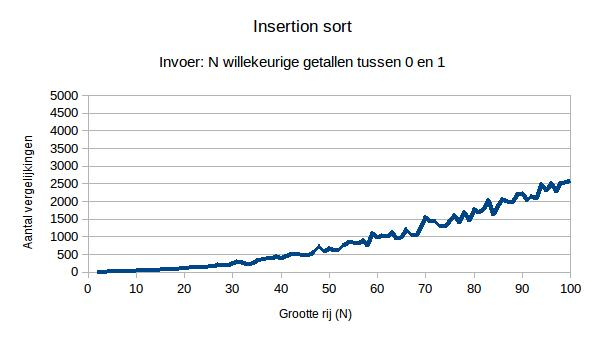
\includegraphics[scale=0.55]{Insertion_1-100.jpg}
\caption{insertion sort}
\label{fig:Insertion_1-100}
\end{figure}

Men ziet dat hoe groter de te sorteren rij is, hoe meer het aantal werkelijke vergelijkingen kan verschillen van het theoretische tilde-model. \newpage

Een schatting voor N=32 000 zou $\approx 32 000^2/4 \approx 256 miljoen $ vergelijkingen geven. Hieronder een doubling ratio experiment van N=2000 tot en met N=32 000.

\begin{figure}[h!]
\centering
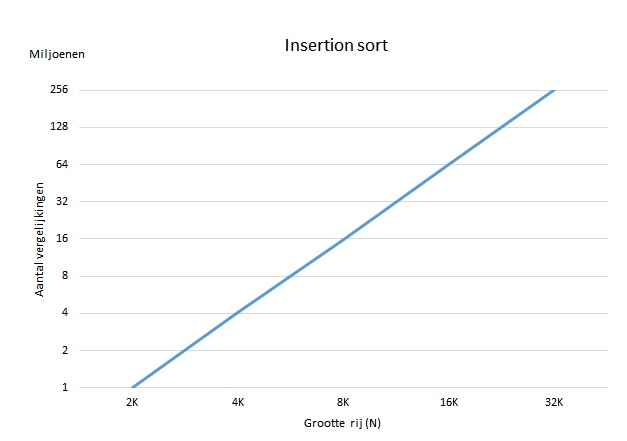
\includegraphics[scale=0.9]{insertion_doubling.jpg}
\caption{Doubling ratio experiment: insertion sort op log-log schaal}
\label{fig:Insertion_doubling}
\end{figure}

De schatting met behulp van de tilde-notatie licht dus relatief dicht bij het werkelijk aantal gemeten vergelijkingen.

\centering{}
\begin{tabular}{| c | c | c |}
\hline
  N & schatting ($N^2/4$) & meting \\
  \hline
  2k & 1M & 1 008 467 \\
  \hline
  4k & 4M & 4 059 042 \\
  \hline
  8k & 16M & 15 966 885 \\
  \hline
  16k & 64M & 63 511 903 \\
  \hline
  32k & 256M & 256 472 004 \\
  \hline
\end{tabular}

\raggedright
Conclusie: de metingen verifiëren de schattingen.

Een belangrijke noot is dat insertion sort in het ideale geval een lineaire tijdscomplexiteit zou kunnen hebben. Dit is het geval indien de rij al gesorteerd zou zijn. Het algoritme zou dan elk element in de rij maar hoeven te "controleren".
\newpage
\subsection{Uitvoeringstijd met behulp van DoublingRatio.java}
Het programma DoublingRatio.java wijst uit dat de doubling ratio voor insertion sort op deze computer nadert naar 4,1 s.

\centering{}
\begin{tabular}{| c | c | c |}
\hline
  N & tijd & doubling ratio \\
  \hline
    2k & 0,0 s & 1,1 \\
  \hline
  4k & 0,0 s & 4,0 \\
  \hline
  8k & 0,2 s & 4,1 \\
  \hline
 16k & 0,7 s & 4,2 \\
  \hline
 32k & 2,8 s & 4,1 \\
  \hline
\end{tabular}

\raggedright
Aan de hand hiervan kunnen we ervan uitgaan dat voor N=64k het sorteren $ 2,8 s * 4,1 = 11,48 s $ zal duren. In praktijk bekomen we: 13,2 s. De schatting klopt dus.

\begin{figure}[h!]
\centering
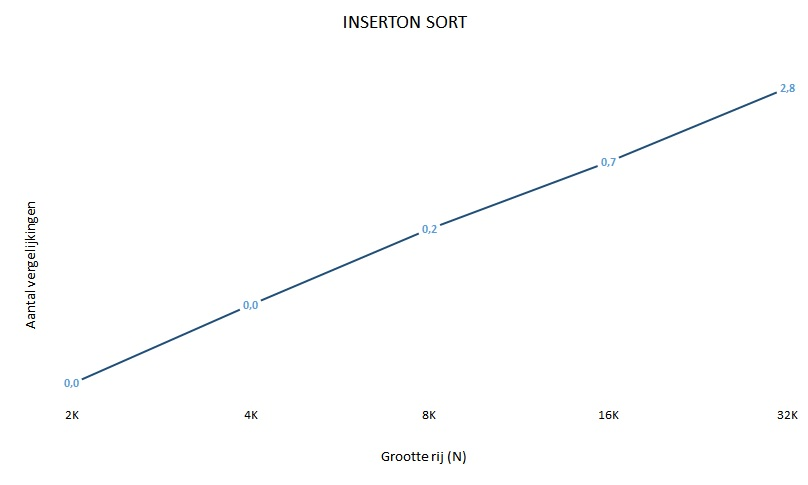
\includegraphics[scale=0.7]{ratio_insertion.jpg}
\caption{Doubling ratio uitvoeringstijd insertion sort}
\label{fig:ratio_insertion}
\end{figure}

\newpage
\section{Quicksort}
Dit sorteer-algoritme werkt door een spil te kiezen in de rij. Dit kan het eerste element, het laatste of een willekeurig element zijn. Uit praktische testen blijkt een willekeurige spil het efficiëntst te zijn. Vervolgens gaat men van links naar rechts zoeken tot men een element vindt dat groter is dan de spil. Vice versa voor de andere richting. Wanneer langs beide kanten van de spil een element groter en kleiner gevonden is aan weerszijden zal men deze van plaats veranderen. Vervolgens doet men hetzelfde voor de deelrij van het eerste element in de rij tot een plaats voor de spil. Alsook voor de deelrij vanaf de spil plus 1 positie tot het einde van de rij. Men doet dit dus steeds 2 keer! Aangezien quicksort zichzelf meerdere malen opnieuw oproept kunnen we stellen dat dit algoritme voornamelijk recursief werkt.

Zoals eerder vermeld roept dit algoritme zichzelf steeds tweemaal op, daarom zal de tijdscomplexiteit met 2 moeten vermenigvuldigt worden. Bij elke oproep naar zichzelf wordt het werk echter door 2 gedeeld. Daarom kunnen we stellen dat dit algoritme logaritmisch werkt. Het partitioneren van de huidige (deelrij) kost daarbij nog eens N tijd. We kunnen dus besluiten dat de tijdscomplexiteit in tilde-notatie $\sim\ 2*N*ln(N)$ is.

\begin{figure}[h!]
\centering
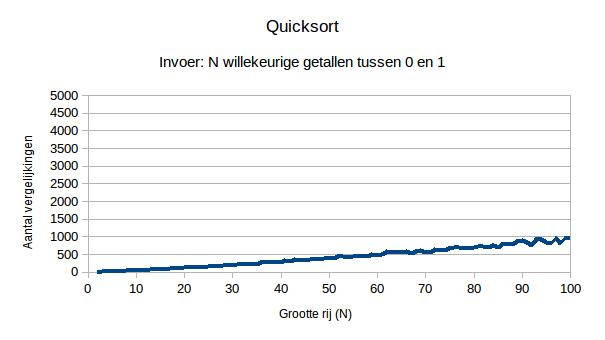
\includegraphics[scale=0.55]{quicksort_1-100.jpg}
\caption{Quicksort}
\label{fig:Quicksort_1-100}
\end{figure}

Figuur \ref{fig:Quicksort_1-100} laat duidelijk zien dat de groei-orde niet kwadratisch is zoals bij insertion sort en selection sort.
\newpage
Een schatting voor N=32 000 zou $\approx 2 * 32 000 * ln(32 000) = 663 duizend $ vergelijkingen geven. Hieronder een doubling ratio experiment van N=2000 tot en met N=32 000.

\begin{figure}[h!]
\centering
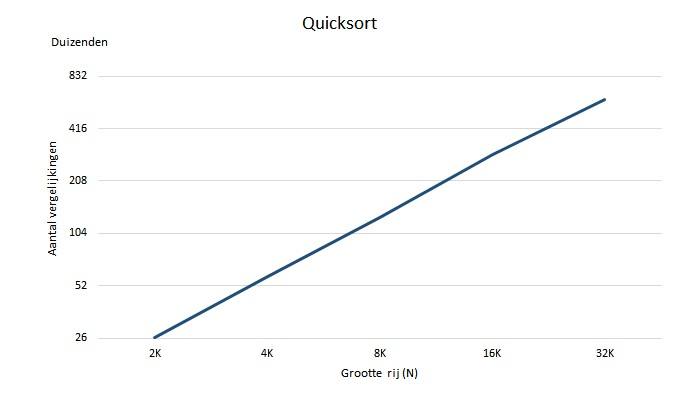
\includegraphics[scale=0.8]{quicksort.jpg}
\caption{Doubling ratio experiment (vergelijkingen): quicksort op log-log schaal}
\label{fig:Quicksort_doubling}
\end{figure}

\centering{}
\begin{tabular}{| c | c | c |}
\hline
  N & schatting ($\sim\ 2*N*ln(N)$) & meting \\
  \hline
  2k & 30 403 & 33 995 \\
  \hline
  4k & 66 352 & 72 035 \\
  \hline
  8k & 143 495 & 155 463 \\
  \hline
  16k & 309 771 & 272 705 \\
  \hline
  32k & 663 903 & 693 215 \\
  \hline
\end{tabular}

\raggedright
Conclusie: de metingen verifiëren de schattingen.
\newpage
\subsection{Uitvoeringstijd met behulp van DoublingRatio.java}
Het programma DoublingRatio.java wijst uit dat de doubling ratio voor quicksort op deze computer nadert naar 2,3.

\centering{}
\begin{tabular}{| c | c | c |}
\hline
  N & tijd & doubling ratio \\
  \hline
  512k & 0,2 s & 2,6 \\
  \hline
1024k & 0,6 s & 2,3 \\
\hline
2048k & 1,2 s & 2,2 \\
\hline
4096k & 2,8 s & 2,3 \\
\hline
8192k & 6,6 s & 2,3 \\
  \hline
\end{tabular}

\raggedright
Aan de hand hiervan kunnen we ervan uitgaan dat N=16 384k, $ 6,6 s * 2,3 = 15,18 s $ zal duren. In praktijk bekomen we: 14,4 s. De schatting klopt dus.

\begin{figure}[h!]
\centering
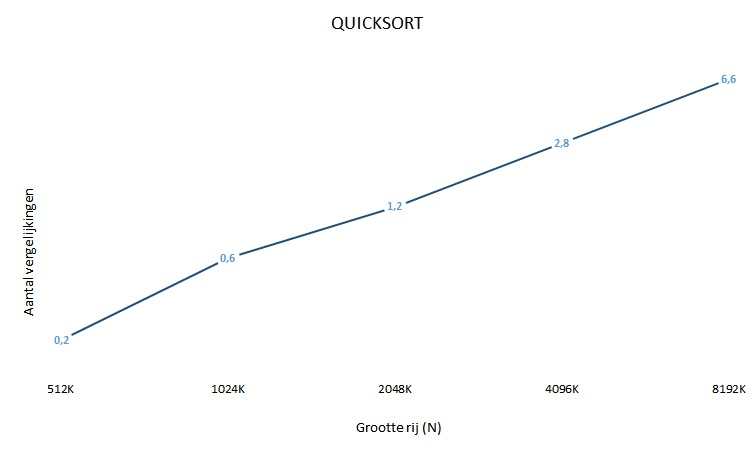
\includegraphics[scale=0.75]{ratio_quick.jpg}
\caption{Doubling ratio uitvoeringstijd quicksort}
\label{fig:ratio_quick}
\end{figure}

\raggedright

\newpage
\section{Selection sort}
Dit sorteer-algoritme werkt door het kleinste element in de volledige rij te zoeken, dit element wordt dan vooraan geplaatst. Dit deel is nu gesorteerd. Het kleinste element van het niet-gesorteerde deel wordt gezocht. Eenmaal gevonden wordt dit opnieuw vooraan in de het ongesorteerde deel geplaatst en zo is dit deel nu ook gesorteerd. Dit gaat verder tot alle elementen in de juiste volgorde staan.

Elke plaats van de rij moet worden ingevuld door het juiste getal, dit brengt al N vergelijkingen op. Vervolgens wordt het ongesorteerde deel van de rij steeds kleiner (N - vordering). Dit levert de volgende tijdscomplexiteit op: $  N + (N-1) + ... + 3 + 2 + 1 = \sim\ N^2/2 $. De deling door 2 is het gevolg dat de rij doorheen het programma de rij voor de helft gesorteerd is waardoor het aantal vergelijkingen ook gehalveerd worden.

\begin{figure}[h!]
\centering
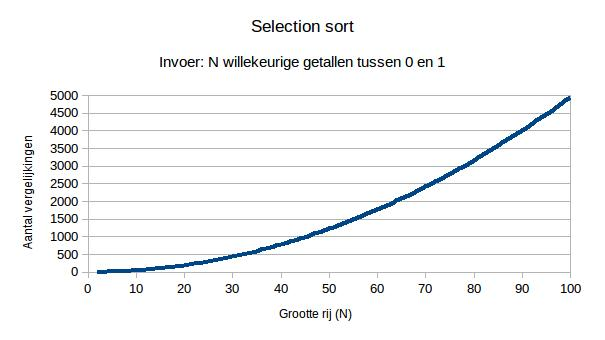
\includegraphics[scale=0.55]{selection_1-100.jpg}
\caption{Selection sort}
\label{fig:Selectiont_1-100}
\end{figure}

Wat opvalt bij dit algoritme is dat het aantal vergelijkingen voor dezelfde lengte van rijen steeds hetzelfde is. Dit is zo omdat deze steeds exact dezelfde (aantal) stappen doet, ongeacht wat de waarden van de elementen van de rij zijn.

\newpage
\section{Vergelijking}
Voor zeer kleine rijen ($N \approx 15$) zijn insertion en selection sort efficiënter. Vanaf dan is quicksort een veel efficiënter sorteer-algoritme. Bij zulke zeer kleine rijen is insertion sort efficiënter dan selection sort, dit ziet men ook terug in de tilde-notatie ($ \sim\ N^2/4 $ voor insertion sort en $ \sim\ N^2/2 $ voor selection sort).

\begin{figure}[h!]
\centering
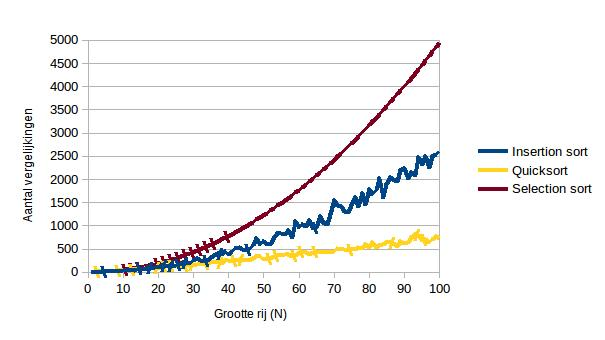
\includegraphics[scale=0.55]{vergelijking.jpg}
\caption{Vergelijking tussen insertion sort, quicksort en selection sort}
\label{fig:Vergelijking}
\end{figure}

\end{document}
